Developers increasingly find themselves as part of a social, connected, online network.
This has its benefits---many developers leverage social media and other online channels to learn about new technology, to stay informed, and to connect with other developers~\cite{singer_software_2014,storey_how_2016}.
In fact, today we see a proliferation of socially-enabled channels~\cite{storey_revolution_2014} through which developers answer each others questions~\cite{mamykina_fastest_2011}, help each other overcome bugs and learn new tools~\cite{parnin_blogging_2013}, and share information in many different forms at many different speeds.
The knowledge and conversations of programmers are increasingly distributed across the web.

About a decade ago, Johnson et al.~\cite{johnson_improving_2005} described how collecting and displaying software telemetry data could help developers make sense of the many streams of measurements one could collect about their software project and process, including build failures, crashes, and source code contributions.
Across builds, coding, and runtime, Johnson et al.\ provided a set of sensors and the metrics they would collect.
Continuous monitoring of diverse signals could enable developers to make better products, with the right interfaces.
For similar reasons, dashboards~\cite{treude_awareness_2010} can help developers keep track of their teammates and checkpoints on software by better capturing thick incoming information in interfaces that integrate well into the development environment.

We propose Johnson et al.'s work is currently missing a category of sensors that is increasingly relevant to clients and maintainers of open source software:
social information on the web.
We concern ourselves with the study of social signals mineable from the web and salient to project clients and maintainers, and the design of interfaces that integrate into the development environment to help developers monitor their projects and choose the right packages.
In this abstract, we focus on the first of these:
a study about what information on the web helps developers answer questions about the social health of open source projects.
We believe this is an important first step to discovering what sensors are the right ones for socially-enabled software telemetry.

\begin{figure*}
\centering
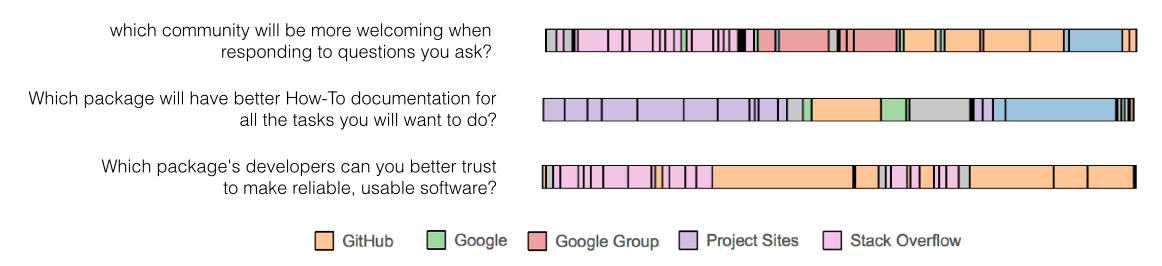
\includegraphics[width=0.9\textwidth]{figures/visits}
\caption{%
The sequence of communication channels one developer visited when answering questions that ask them to compare the quality of packages' community, documentation, and developers.
Though we have found that users often rely on different channels, though this one relies on an interesting assortment:
project documentation, GitHub, and blog posts to learn about the availale How-To documentation;
Stack Overflow, Reddit, and Google Groups to learn about how welcoming the community is;
GitHub profile pages, issues, pull request, and Stack Overflow to learn more about the developers behind the package.
}
\label{fig:visits}
\end{figure*}

There are several online tools we see as precursors to much more powerful socially-enabled telemetry systems.
%Slant\footnote{\url{http://www.slant.co/}} allows developers to request comparisons of alternatives of packages for programming tasks like drawing libraries and package managers through bite-sized bullet point pros and cons written by peers.
Awesome Python\footnote{\url{https://python.libhunt.com/}} generates comparisons of arbitrary pairs of Python packages\footnote{\url{https://python.libhunt.com/project/pygame/vs/panda3}}, with popularity and activity metrics presumably based on download counts and commit activity.
Ruby Toolbox\footnote{\url{https://www.ruby-toolbox.com/}} and the `packagequality' widget\footnote{\url{http://packagequality.com/}} compute package quality ratings that draw on download counts, responses to issues, and GitHub stars.
While these can be proxies for a package's quality, we believe that this isn't enough for understanding the social life of packages.
When using packages, developers are concerned with the trustworthiness of developers~\cite{robillard_field_2011}, how up-to-date the documentation is~\cite{storey_revolution_2014,nykaza_what_2002,lethbridge_how_2003,robillard_field_2011}, and whether the community is anti-social~\cite{storey_revolution_2014}.

As developers will often have to make trade-offs between these factors when choosing software, we are skeptical that anything short of carefully selected and arranged samples from socially-enabled channels can help a developer make a truly informed judgment about a package's community when evaluating software and, after on-boarding, choosing how to ask for help.
This abstract presents our inquiry into what these samples from developers' socially-enabled networks and web pages should be.

\if 0
Software developers decide to reuse software to save time~\cite{mili_reusing_1995}.
Researchers have observed that given a task, developers can assemble working programs through components found entirely on the web, together with their prior knowledge (e.g.,~\cite{brandt_two_2009}).
This behavior is not uncommon---foraging for information online has been observed in particular for a variety of non-professional programmers~\cite{brandt_opportunistic_2008} and validated through the queries for a help search engine for developer tools~\cite{brandt_two_2009}.

Though there are hazards in how developers select reusable components for software in practice.
A premium is placed on working source code examples~\cite{nykaza_what_2002}.
Developers' tend to choose code that ``satisfices'' without thoroughly testing it~\cite{brandt_two_2009}.
APIs have unexpected and undocumented side effects~\cite{robillard_field_2011}.
And despite a rise of ``socially enabled'' digital media for communicating about software, programmers face challenges using these channels:
they may be overwhelmed by the amount of content and distrust its quality~\cite{storey_revolution_2014}.

In this study, we present a view of how developers learn about packages on socially enabled channels.
Through this study, we highlight two problems:
First, programmers attempt to make sense of distributed information online.
Second, some information is hidden from view, only to be discovered after tens of minutes of inspection.
For us, these findings will motivate the design of new search systems for developers looking for resuable software components.
\fi

% We believe that such representations, shown in the right place when developers are choosing new components, reduce the hazards of poor reuse choices when developers lack media literacy, and can help programmers understand what components are safe to trust.

\if 0
The past five decades of software engineering have seen the rise of digital media for programmer communication and information sharing.
As of the '90s, the web has ``socially enabled'' many new digital media, transforming how developers learn about new technologies~\cite{storey_revolution_2014}.
In the last ten years, millions of projects migrated to GitHub, a social code hosting site, and hundreds of thousands of packages of reusable software have been published on globally available and instantly accessible ``package indexes'' for the Ruby, JavaScript, and Python languages.
Not only has reusable software moved online en masse, but so too has much of the documentation for this work.

In this paper, we describe how indications of content quality can be harvested on a package level from four top digital channels that developers use for development~\cite{storey_revolution_2014}, three of which are socially enabled: code hosting, Q\&A sites, web search, and micro-blogging.
We focus specifically on reusable components at the resolution of packages, or self-contained libraries that can be installed from a package index and easily imported into one's code.
We make this choice as packages have a system image that, although distributed and ``fragmented,'' is accessible through thoughtful and systematized queries to the search interfaces and APIs of social media and web search.

Our primary contribution is that we build a system that creates summaries of package support quality by collecting fragmented information across digital channels and summarizes them in lightweight representations.
We report how developers perceive the trustworthiness of software given these representations.
We then suggest which channels appear to be the richest for conveying variation on the quality of reusable components to developers who have not seen them before.
We present several example interfaces that show how these indications can be incorporated into modern interfaces where programmers seek help and may encounter the option to install packages.
\fi
